\section{Research Method}\label{sec-research-method}
Ethnography is a \textit{participant observation} method. It does not interfere (beyond the ethnographic researchers' presence) with the observed ESE researchers' "life" \cite{Sharp-2016-Ethnographic-Studies-ESE}. Ethnographic researchers adopt "the ESE researchers' point of view" to better understand the reason for their actions \cite[pp. 55-56]{Outhwaite-2007-sage}. Thus, the biases and misperceptions that ESE researchers might have about themselves can be detected. Ethnography also captures the rich context that surrounds ESE researchers.

Ethnography identifies details that are ignored by or in other methods. The disadvantage is the time required for learning \cite{Sharp-2016-Ethnographic-Studies-ESE}. Thus, we opted to study a single experimental research group over a long period instead of working halfway with several experimental research groups over shorter periods. This decision was also motivated by the challenge of finding several open-minded experimental research groups willing to participate in this research. We selected a representative, i.e., respected and well-known, research group to guarantee (to the extent possible) the reliability of the results, their validity, and the findings' scientific significance \cite{sjoberg-2007-future-empical-methods}.

We followed Runenson et al.'s case study guidelines \cite{Runenson-2012-case-study-SE} wherever they apply to ethnographical studies. Our research protocol is organized along three axes:

\begin{itemize}
	\item \textbf{Context selection}, i.e., choose the experimental research group that facilitates the research in the best possible condition.
    \item \textbf{Data collection procedures}.
    \item \textbf{Data analysis procedures}.
\end{itemize}

To avoid confusion, from this point on, we will refer to the "ESE researchers" with whom we interact during the investigation as "the experimenters". We will talk about ourselves, the authors, as "the researchers". We, authors/researchers, play two different roles in the investigation:

\begin{itemize}
\item \textbf{Efra\'in R. Fonseca C.} and Edison G. Espinosa conducted the ethnographic study as part of their Ph.D. Edison G. Espinosa abandoned the ethnographic study early (during the investigation reported in Section~\ref{replication}) and changed the orientation of his Ph.D. This is the reason he is not authoring this paper. The personal opinions poured in Section~\ref{sec-reseach-execution} belong to these two researchers, particularly Efra\'in R. Fonseca C.
\item \textbf{Oscar Dieste} and \textbf{Natalia Juristo} supervised the investigation. Their views and opinions are not reflected in this manuscript.
\end{itemize}

\subsection{Context selection}
We have considered an experimental research group as "representative," i.e., a reliable source of information when it fulfills the following selection criteria:

\begin{itemize}
	\item The experimental research group has extensive experience in ESE research.
	\item The ESE community recognizes the experimenters as specialists in their areas.
	\item The group has many publications in journals of repute and internal documentation, i.e., the group has a verifiable track record.
\item One of the main drivers of this research is to explore the connection between replication and lab practices. We positively value that the experimental research group conducts replications or families of experiments.
\end{itemize}

Based on these criteria, we selected an experimental research group with more than 20 years of experience in experimentation in SE. The experimenters have a long track record of publication in journals and conferences of repute. The group has focused on replications and families of experiments since they consider that isolated experiments do not contribute significantly to scientific knowledge. The manuscript conceals the group's identity but is disclosed in the raw data repository (see Section \ref{sub-sec-research-documentaition}).

\subsection{Data collection procedures}\label{subsec-data-collection}

The information sources within the experimental research group under study (RGUS) are:

\begin{itemize}

	\item Experimenters' knowledge.
	
	\item General and specific literature, e.g., the book \textquotedblleft Experimentation in Software Engineering\textquotedblright~\cite{Wohlin-2012-experimentatio-SE}.
	
	\item General and specific experimental materials, e.g., experimental designs.
	
	\item Periodic and/or \textit{ad-hoc} activities carried out, e.g., experimental planning.
	
\end{itemize}

Ethnography information gathering is characterized by being cyclical, iterative, and incremental. The data acquisition process was based on a taxonomy of information-gathering techniques, categorized according to the level of contact with the primary source of information. Such a taxonomy proposes three levels of information gathering: direct participation with the source (level 1), indirect participation with the source (level 2), and study of the experiment material without the participation of the source (level 3) \cite{Lethbridge-2005-data-collection-techniques-SE}. Table \ref{tbl-tecnica-fuente} describes the information-gathering techniques and instruments and the corresponding information sources to which they can be applied.

\begin{table}
	\small
	\centering
	\caption{Techniques and tools for information acquisition, by source}
	\label{tbl-tecnica-fuente}
	\begin{tabular}{|p{2cm}|p{2.5cm}|p{3cm}|}
	\hline
	\textbf{Source} & \textbf{Technique} & \textbf{Instruments}\\
	\hline
	\multirow{14}{50 pt}{Experimenters knowledge} & Interviews & Video camera, paper, pencil\\
	\cmidrule{2-2}\cmidrule{3-3}
	& Focus groups & Video camera, blackboard, cardboard, board markers, chalkboard eraser, etc.\\
	\cmidrule{2-2}\cmidrule{3-3}
	& Process modeling & Video camera, paper, pencil\\
	\cmidrule{2-2}\cmidrule{3-3}
	& Instrumental systems & Email, videoconferences, internet\\
	\cmidrule{2-2}\cmidrule{3-3}
	& Experience-based learning & Literature review, review of experimental material, experimentation in practice\\
	\hline
	\multirow{4}{15 pt}{Common literature} & Documentation analysis & Comprehensive reading of literature, reading summaries, software support tools\\
	\hline
	\multirow{3}{15 pt}{Experimental material} & Documentation analysis & Systematic analysis of experimental material, trials with data\\
	\hline
	\multirow{2}{15 pt}{Group activities} & Participatory observation & Literature review, researchers knowledge\\
	\hline
	\end{tabular}
\end{table}

The order in which researchers contact information sources is random. The frequency of contact depends on the researchers' need to answer research questions during the ethnographic research and the availability of each source. 

\subsection{Data analysis procedure}

The ethnographic practice involves storing the raw data and then interpreting the findings \cite{Cooper-2007-Sharing-Data-Ethnographic-Research}. In this research, the data analysis procedure consists of four activities:

\begin{itemize}
\item \textbf{Preparation of materials}: The information sources are classified and categorized so experimenters and researchers can manage them.
\item \textbf{Information acquisition}: While analyzing the information sources, researchers gradually acquire basic knowledge about experimentation, which helps them understand the experimenters' knowledge and behavior more easily.
\item \textbf{Verification of information}: This is probably the most complex activity. The knowledge obtained from the sources complements each other. We will use triangulation to explain the findings and identify new areas of inquiry. All findings are discussed with the experimenters to avoid misunderstandings and verify that the resulting activities are those that they carry out in practice.
\item \textbf{Generation of results}: Finally, we obtained the results as final products after several iterations of comparison, verification, and consensus between researchers and experimenters. The expected results will be models (conceptual and process) and practices derived from the interviews with the experimenters.
\end{itemize}

\subsection{Research documentation}\label{sub-sec-research-documentaition}
The raw data obtained in this study is organized as shown in Figure \ref{fig-info-study}. The tree represents a repository of around 20GB of information. The repository contains pictures, recordings, models, reports, and transcriptions, most in Spanish (the operational language used during the research). Spanish is widespread enough to utilize the repository with little effort. The final products, e.g., models, have been translated into English to improve the reader's understanding. The repository is not public because it contains personal data. However, upon request, the corresponding author will share the repository with interested researchers.

\begin{figure}[htbp!]
	\centering
	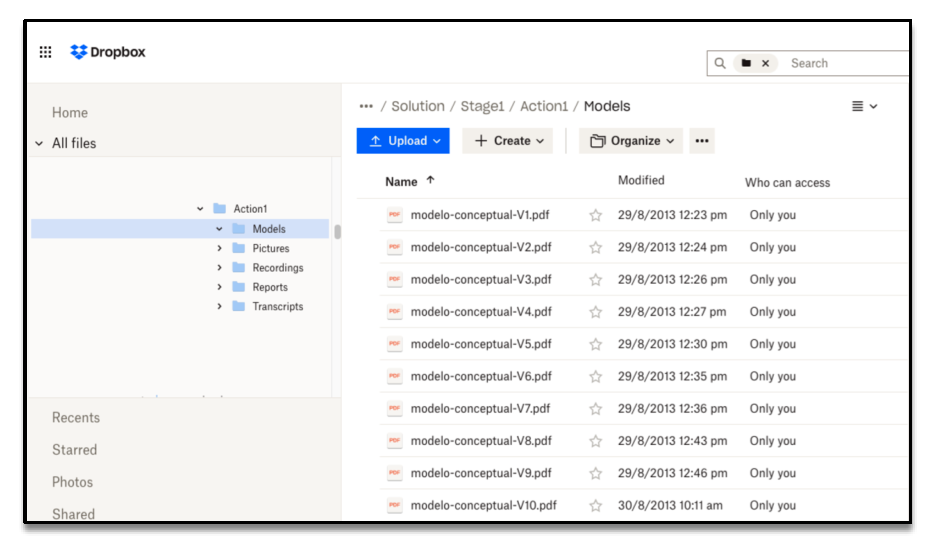
\includegraphics[width=\columnwidth]{images/Intermediate-Products}
	\caption{Repository structure}
	\label{fig-info-study}
\end{figure}
